% method-our-model.tex
%
% Drafted by Juntang on August 22, 2024
% Adj T on Sep 23, 24

\begin{frame}
  \frametitle{Our Model}
    \begin{columns}
        \column{0.68\textwidth}
        \begin{block}{}
        \begin{equation}
            \Leftrightarrow \sigma \frac{dC_{i}(t)}{dt} + C_{i}(t) = C_{i-1}(t-AT) u(t-AT)
        \end{equation}
        \begin{equation}  
            \begin{aligned}
                R(t) = C_n(t) &= {\left\{
                \begin{array}{ll}
                \frac{t^\alpha}{\Gamma(\alpha+1)\sigma^{\alpha+1}} e^{-\frac{t - AT_1}{\sigma_1}}, & \text{if } t \geq AT_1 \\
                0, & \text{otherwise}
                \end{array}
                \right.}
            \end{aligned}
        \end{equation}
        \vspace{-13pt}
        \begin{enumerate}
            \item $C_{AIF} \rightarrow C_{in}$:
            \begin{equation}
                C_{in}(t) = \frac{k_H}{\kappa} \left( C_{AIF} * R_{1}^{[P]} \right)(t)
            \end{equation}
            %
            \item $C_{in} \rightarrow C_{tissue}$:
            \begin{equation}
            C_{tissue}(t) = \left( C_{in} * R_{2} \right)(t)
            \end{equation}

            \item[] where:
            
            $\begin{aligned}
                k_H &= \left(\frac{1 - H_{LV}}{1 - H_{SV}}\right) \\
                \kappa &= \int_0^T C_a(\tau) d\tau / \int_0^T C_v(\tau) d\tau
            \end{aligned}$    
            
        \end{enumerate}
        \end{block}

        \hspace*{4em}  

        \column{0.23\textwidth}
        \begin{figure}[h]
            \centering
            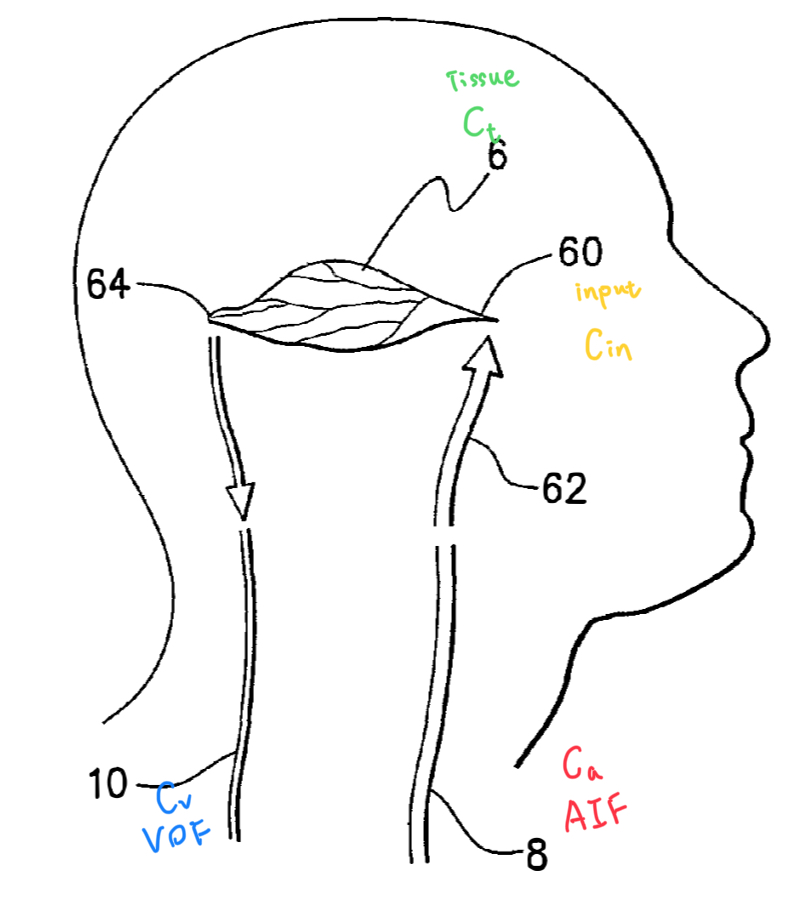
\includegraphics[width=\textwidth]{figures/method-our.jpeg}
            \caption{Diagram of the system illustrating the different concentrations involved in the model. \(C_a\) (red) represents the arterial input function (AIF), \(C_{in}\) (yellow, imaginary) represents the entrance concentration, \(C_t\) (green) represents the tissue concentration, and \(C_v\) (blue) represents the venous output function (VOF). }
            \label{fig:solution_plot}
        \end{figure}
        
        
    \end{columns}
   

\end{frame}

%%% Local Variables:
%%% mode: latex
%%% TeX-master: "../topic-slide-main"
%%% End: